\documentclass[aspectratio=169, xcolor=dvipsnames]{beamer}

\useoutertheme{miniframes}
\useinnertheme{circles}
\usepackage{appendixnumberbeamer}
\setbeamertemplate{footline}[frame number]

\definecolor{main_color}{HTML}{7D9D33}
\definecolor{secondary_color}{HTML}{CED38C}

\setbeamercolor{palette primary}{bg=secondary_color,fg=white}
\setbeamercolor{palette secondary}{bg=secondary_color,fg=white}
\setbeamercolor{palette tertiary}{bg=secondary_color,fg=white}
\setbeamercolor{palette quaternary}{bg=secondary_color,fg=white}
\setbeamercolor{structure}{fg=main_color}
\setbeamercolor{section in toc}{fg=secondary_color}
\setbeamercolor{subsection in head/foot}{bg=main_color,fg=white}

\usepackage{booktabs}
\usepackage{graphicx}
\usepackage{subcaption}
\usepackage{caption}

\graphicspath{{./reference_pics/}{/Users/ohouck/globus/forecast_data/figures/}}

\title{Tailoring Machine Learning Weather Predictions for Local Impacts}
\author{\textbf{Ozma Houck, James Franke}}
\date{}

\usepackage{bbm}


\usepackage[round]{natbib}
\bibliographystyle{aer}

\begin{document}

\maketitle

\section{Background}

\begin{frame}{What's Been Happening in Weather Forecasting?}
    \begin{columns}[T]
        \begin{column}{0.58\textwidth}
            \begin{itemize}
                \item Traditional numerical weather prediction (NWP) models are expensive and slow to run.
                %These are physics based models which create predictions by solving the PDE's that govern the atmosphere.
                \begin{itemize}
                    \item Ex: Best global weather model created by European Centre for Medium-Range Weather Forecasts (ECMWF) requires a supercomputer.
                \end{itemize}
                \item<2-> Beginning in 2022, several machine learning (ML) based weather models have been created that have rivaled or exceeded the accuracy of traditional models.
                \item<2-> Instead of requiring a supercomputer, these models can be run on a personal laptop.
            \end{itemize}
        \end{column}
        \begin{column}{0.38\textwidth}
            \vspace{0.5cm}
            \begin{figure}
                \centering
                \includegraphics<1-2>[width=\linewidth]{ECMWF_supercomputer.png}
                \caption*{\small ECMWF Supercomputer}
            \end{figure}
        \end{column}
    \end{columns}
\end{frame}

\begin{frame}{Increased Accessibility of Weather Predictions Opens New Opportunities}
    \begin{itemize}
        \item Global models are more accurate in some areas than others.
        \item Different groups prioritize accuracy for different weather variables.
        \item Low compute requirements for creating ML weather forecasts offer the potential to help democratize access to accurate weather predictions.
    \end{itemize}
        
    \pause
    \begin{itemize}
        \item \textbf{The Problem:} All global weather models (NWP and ML) are trained to optimize overall global accuracy.
        \begin{itemize}
            \item A temperature error in Greenland is treated the same as a temperature error in Chicago!
            \item The ML models might be cheap to run, but they are extremely expensive to train!
        \end{itemize}
     \item \textbf{Potential Solution:} Post-process (fine-tune) global model outputs with a small, localized model to improve accuracy for specific regions and weather variables of interest. 
    \end{itemize}
\end{frame}

\begin{frame}{Accurate weather forecasts matter and post-processing can improve accuracy}
    \textbf{Why Accurate Weather Forecasts Matter:}
    \begin{itemize}
        \item Accurate temperature forecasts reduce heat mortality. (Shrader et al. 2023)
        \item Renewable forecast errors increase electricity prices and thermal generator start-ups. (Weber and Woerman 2024)
        \item Monsoon onset forecasts can help farmers adjust planting dates. (Burlig et al. 2025)
    \end{itemize}

    \textbf{Prior Work on Post-Processing Weather Forecasts:}
    \begin{itemize}
        \item Neural networks can be used to post-process NWP models. (Rasp and Lerch 2018)
        \item CNNs can be used to correct NWP models on gridded data. (Han et al. 2021) 
        \item NWP and ML models can be post-processed in a similar process-based model (Trotta et al. 2025). 
    \end{itemize}
\end{frame}

\begin{frame}{How to Post-Process Weather Model Outputs? What Outputs Matter Most?}

    \begin{itemize}
        \item \textbf{Contribution 1}: Demonstrate that a simple low-compute neural network model can meaningfully improve the accuracy of both traditional and ML weather models and show where these simple models perform well, and where they struggle. (Main Results Today)
        \item \textbf{Contribution 2}: Show that post-processing using alternative loss functions can lead to greater improvements for specific weather variables of interest.(In Progress)
        \item \textbf{Contribution 3}: Using agriculture as a test case, demonstrate how damage functions can be estimated and incorporated as custom loss functions when post-processing. (In Progress)
    \end{itemize}
\end{frame}

\section{How to Post-Process?}


\begin{frame}{Fine-Tuning Approach}
    \hypertarget{FineTuning}{} % target for returning from appendix
    \textbf{Data:}
    \begin{itemize}
        \item Forecast predictions from IFS (NWP) and Pangu (ML) Global Models (0.25 degree resolution)
        \item Ground truth data from ERA5 Reanalysis (0.25 degree resolution)
        \item Focus on 2m Temperature and 10m Wind Speed
    \end{itemize}

    \textbf{Model:}
    \begin{itemize}
        \item Train a post-processing neural network for a specific variable in a specific region.
        \item Loss Function: Mean Squared Error (MSE)
        \item Test simple multi-layer perceptron (MLP) and convolution based UNET architectures.
    \end{itemize}
% button to go to appendix slide with training details
\hyperlink{TrainingDetails}{\beamerbutton{Training Details}}
\hyperlink{Neural Net Background}{\beamerbutton{Neural Net Background}}
\end{frame}
    

\begin{frame}{Start by Manually Looking at Five Regions of Interest}
    \begin{itemize}
        \item Manually choose a few regions with a variety of climates and land terrains. 
        \item Sample from different climate zones (arid, temperate, tropical). 
        \item Sample from different topographic zones (coastal, mountainous, flat).
    \end{itemize}
    
    \begin{figure}
        \centering
        \includegraphics[width=0.8\linewidth]{climate_zones_with_patches.png}
    \end{figure}
\end{frame}
\begin{frame}{Start by Manually Looking at Five Regions of Interest}
    \begin{itemize}
        \item Manually choose a few regions with a variety of climates and land terrains. 
        \item Sample from different climate zones (arid, temperate, tropical). 
        \item Sample from different topographic zones (coastal, mountainous, flat).
    \end{itemize}
    
    \begin{figure}
        \centering
        \includegraphics[width=0.8\linewidth]{topo_zones_with_patches.png}
    \end{figure}
\end{frame}

\begin{frame}{See Greater Improvements for Longer Lead Times and for Wind Speed}
    \begin{figure}
        \centering
        \begin{subfigure}[t]{0.48\textwidth}
            \centering
            \includegraphics[width=\linewidth]{pangu/lead_time/multi_region/6x6/leadtime_rmse_improvement_2m_temperature_trainedwith_2m_temperature_geographic_pangu_mlp.png}
            \caption{2m Temperature: Pangu (ML Model)}
        \end{subfigure}
        \hfill
        \begin{subfigure}[t]{0.48\textwidth}
            \centering
            \includegraphics[width=\linewidth]{pangu/lead_time/multi_region/6x6/leadtime_rmse_improvement_10m_wind_speed_trainedwith_10m_wind_speed_geographic_pangu_mlp.png}
            \caption{Wind Speed: Pangu (ML Model)}
        \end{subfigure}
    \end{figure}
\end{frame}

\begin{frame}{Similar Performance When Using NWP Model (IFS) Outputs}
    \begin{figure}
        \centering
        \begin{subfigure}[t]{0.48\textwidth}
            \centering
            \includegraphics[width=\linewidth]{ifs/lead_time/multi_region/6x6/leadtime_rmse_improvement_2m_temperature_trainedwith_2m_temperature_geographic_ifs_mlp.png}
            \caption{2m Temperature: IFS (NWP Model)}
        \end{subfigure}
        \hfill
        \begin{subfigure}[t]{0.48\textwidth}
            \centering
            \includegraphics[width=\linewidth]{ifs/lead_time/multi_region/6x6/leadtime_rmse_improvement_10m_wind_speed_trainedwith_10m_wind_speed_geographic_ifs_mlp.png}
            \caption{Wind Speed: IFS (NWP Model)}
        \end{subfigure}
    \end{figure}
\end{frame}

\begin{frame}{Slightly Better Performance for UNet vs MLP}
    \begin{figure}
        \centering
        \begin{subfigure}[t]{0.48\textwidth}
            \centering
            \includegraphics[width=\linewidth]{pangu/lead_time/multi_region/6x6/leadtime_rmse_improvement_2m_temperature_trainedwith_2m_temperature_geographic_pangu_unet.png}
            \caption{2m Temperature: Pangu (ML Model)}
        \end{subfigure}
        \hfill
        \begin{subfigure}[t]{0.48\textwidth}
            \centering
            \includegraphics[width=\linewidth]{pangu/lead_time/multi_region/6x6/leadtime_rmse_improvement_10m_wind_speed_trainedwith_10m_wind_speed_geographic_pangu_unet.png}
            \caption{Wind Speed: Pangu (ML Model) using UNet}
        \end{subfigure}
    \end{figure}
\end{frame}

\begin{frame}{Post-processing lessens systematic biases in forecasts}
    
    Over correcting temperature bias in India.
    \begin{figure}
        \centering
        \begin{subfigure}[t]{0.48\textwidth}
            \centering
            \includegraphics[width=\linewidth]{pangu/lead_time/multi_region/6x6/leadtime_raw_values_2m_temperature_trainedwith_2m_temperature_geographic_pangu_mlp.png}
            \caption{Raw 2m Temperature Forecast Error: Pangu (ML Model)}
        \end{subfigure}
        \hfill
        \begin{subfigure}[t]{0.48\textwidth}
            \centering
            \includegraphics[width=\linewidth]{pangu/lead_time/multi_region/6x6/leadtime_raw_values_10m_wind_speed_trainedwith_10m_wind_speed_geographic_pangu_mlp.png}
            \caption{Raw 10m Wind Speed Forecast Error: Pangu (ML Model)}
        \end{subfigure}
    \end{figure}
\end{frame}

\begin{frame}{Lower likelihood of large errors after post-processing}
    \begin{figure}
        \centering
        \begin{subfigure}[t]{0.48\textwidth}
            \centering
            \includegraphics[width=\linewidth]{pangu/lead_time/multi_region/6x6/leadtime_error_cutoff_2m_temperature_trainedwith_2m_temperature_geographic_pangu_mlp.png}
            \caption{Share of 2m Temperature Errors Above 2°C: Pangu (ML Model)}
        \end{subfigure}
        \hfill
        \begin{subfigure}[t]{0.48\textwidth}
            \centering
            \includegraphics[width=\linewidth]{pangu/lead_time/multi_region/6x6/leadtime_error_cutoff_10m_wind_speed_trainedwith_10m_wind_speed_geographic_pangu_mlp.png}
            \caption{Share of 10m Wind Speed Errors Above 2 m/s: Pangu (ML Model)}
        \end{subfigure}
    \end{figure}
\end{frame}

\begin{frame}{Climate Zones}
    \begin{figure}
        \centering
        \begin{subfigure}[t]{0.48\textwidth}
            \centering
            \includegraphics[width=\linewidth]{pangu/lead_time/multi_region/2x2/leadtime_rmse_improvement_2m_temperature_trainedwith_2m_temperature_climate_zones_pangu_mlp_bootstrap.png}
            \caption{2m Temperature: Pangu}
        \end{subfigure}
        \hfill
        \begin{subfigure}[t]{0.48\textwidth}
            \centering
            \includegraphics[width=\linewidth]{pangu/lead_time/multi_region/2x2/leadtime_rmse_improvement_10m_wind_speed_trainedwith_10m_wind_speed_climate_zones_pangu_mlp_bootstrap.png}
            \caption{Wind Speed: Pangu}
        \end{subfigure}
    \end{figure}
\end{frame}

\begin{frame}{Topographic Zones}
\begin{figure}
    \centering
    \begin{subfigure}[t]{0.48\textwidth}
        \centering
        \includegraphics[width=\linewidth]{pangu/lead_time/multi_region/2x2/leadtime_rmse_improvement_2m_temperature_trainedwith_2m_temperature_topographic_zones_pangu_mlp_bootstrap.png}
        \caption{2m Temperature: Pangu}
    \end{subfigure}
    \hfill
    \begin{subfigure}[t]{0.48\textwidth}
        \centering
        \includegraphics[width=\linewidth]{pangu/lead_time/multi_region/2x2/leadtime_rmse_improvement_10m_wind_speed_trainedwith_10m_wind_speed_topographic_zones_pangu_mlp_bootstrap.png}
        \caption{Wind Speed: Pangu}
    \end{subfigure}
\end{figure}
\end{frame}


\section{Custom Loss Functions}

\begin{frame}{All Deterministic Forecasts Trained with MSE, All Ensemble Models Trained with CRPS}
    \begin{itemize}
        \item Under-prediction errors of extreme temperatures have a disproportionate impact on mortality rates.
        \item Temperature errors around freezing point have outsized impacts on agriculture.
        \item Wind speed errors during high wind events have larger impacts on wind power generation than errors during calm periods.
    \end{itemize}
    \textbf{Question:} If we know the damage function of different types of errors, can we use custom loss functions to meaningfully improve accuracy for these impactful errors while still maintaining overall accuracy?
\end{frame}

\begin{frame}{Version 0: Damage Weighted MSE Loss Function}
    \begin{figure}
        \centering
        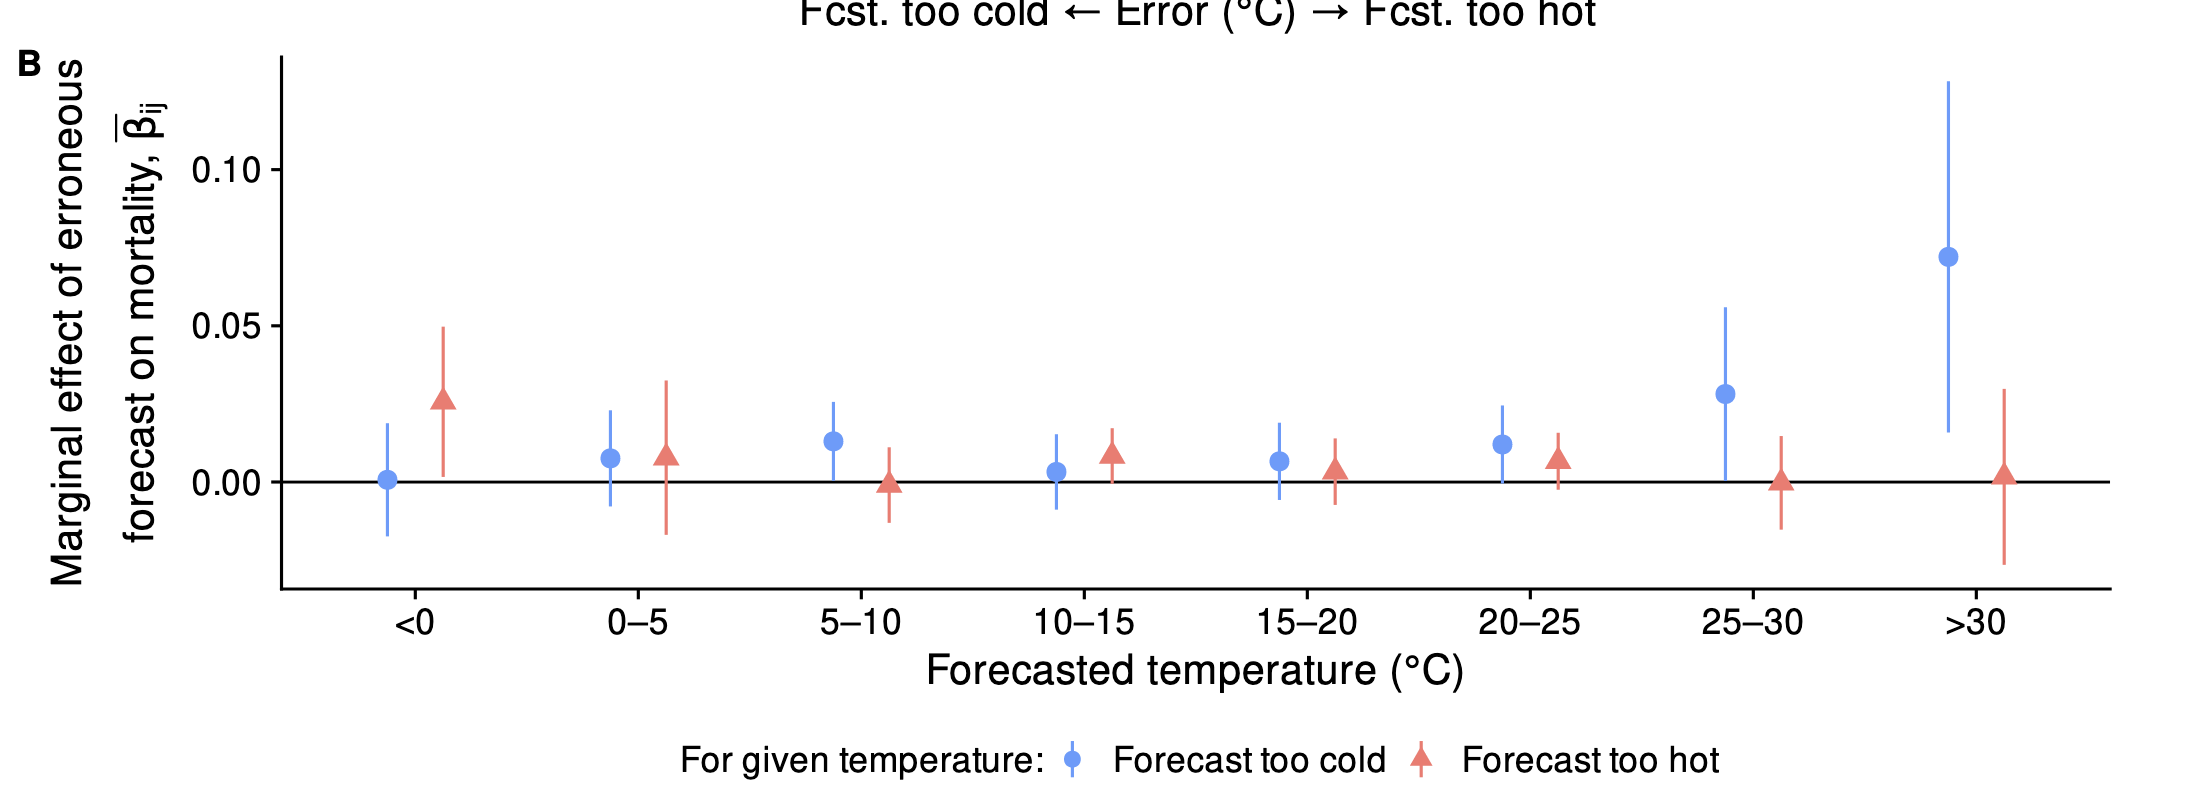
\includegraphics[width=0.6\linewidth,keepaspectratio]{mortal_errors_fig.png}
        \caption*{\small From Shrader et al. 2023 }
    \end{figure}
\end{frame}

\begin{frame}{Able to improve performance based on damage weighted MSE}
    \begin{columns}[T]
        \begin{column}{0.48\textwidth}
            \vspace{0.5cm}
            \begin{figure}
                \centering
                \includegraphics[width=\linewidth]{pangu/lead_time/multi_region/6x6/leadtime_rmse_improvement_2m_temperature_trainedwith_2m_temperature_geographic_pangu_extreme_heat_mlp.png}
                \caption*{\small Pangu: Extreme Heat Trained Model (Damage Weighted MSE)}
            \end{figure}
        \end{column}
        \begin{column}{0.48\textwidth}
            \vspace{0.5cm}
            \begin{figure}
                \centering
                \includegraphics[width=\linewidth]{pangu/lead_time/multi_region/6x6/leadtime_rmse_improvement_2m_temperature_trainedwith_2m_temperature_geographic_pangu_mlp.png}
                \caption*{\small Pangu: Original Unweighted MSE }
            \end{figure}
        \end{column}
    \end{columns}
\end{frame}

\begin{frame}{Able to improve performance based on damage weighted MSE}
    \begin{columns}[T]
        \begin{column}{0.48\textwidth}
            \vspace{0.5cm}
            \begin{figure}
                \centering
                \includegraphics[width=\linewidth]{pangu/lead_time/multi_region/6x6/leadtime_rmse_improvement_2m_temperature_trainedwith_2m_temperature_geographic_pangu_extreme_heat_mlp.png}
                \caption*{\small Pangu: Extreme Heat Trained Model (Damage Weighted MSE)}
            \end{figure}
        \end{column}
        \begin{column}{0.48\textwidth}
            \vspace{0.5cm}
            \begin{figure}
                \centering
                \includegraphics[width=\linewidth]{pangu/lead_time/multi_region/6x6/leadtime_rmse_improvement_2m_temperature_trainedwith_2m_temperature_geographic_pangu_extreme_heat_train_rmse_eval_mlp.png}
                \caption*{\small Pangu: Unweighted RMSE on Extreme Heat Trained Model}
            \end{figure}
        \end{column}
    \end{columns}
\end{frame}

\begin{frame}{Comes at the cost of overall raw error performance in some regions}
    \begin{columns}[T]
        \begin{column}{0.48\textwidth}
            \vspace{0.5cm}
            \begin{figure}
                \centering
                \includegraphics[width=\linewidth]{pangu/lead_time/multi_region/6x6/leadtime_raw_values_2m_temperature_trainedwith_2m_temperature_geographic_pangu_extreme_heat_mlp.png}
                \caption*{\small Pangu: Extreme Heat Trained Model Raw 2m Temperature Error}
            \end{figure}
        \end{column}
        \begin{column}{0.48\textwidth}
            \vspace{0.5cm}
            \begin{figure}
                \centering
                \includegraphics[width=\linewidth]{pangu/lead_time/multi_region/6x6/leadtime_raw_values_2m_temperature_trainedwith_2m_temperature_geographic_pangu_mlp.png}
                \caption*{\small Pangu: Original Model Raw 2m Temperature}
            \end{figure}
        \end{column}
    \end{columns}
\end{frame}
\begin{frame}{However, no real cost when looking at large error share}
    \begin{figure}
        \centering
        \begin{subfigure}[t]{0.48\textwidth}
            \centering
            \includegraphics[width=\linewidth]{pangu/lead_time/multi_region/6x6/leadtime_error_cutoff_2m_temperature_trainedwith_2m_temperature_geographic_pangu_extreme_heat_mlp.png}
            \caption*{\small Pangu: Extreme Heat Trained Model Share of 2m Temperature Errors Above 2°C}
        \end{subfigure}
        \hfill
        \begin{subfigure}[t]{0.48\textwidth}
            \centering
            \includegraphics[width=\linewidth]{pangu/lead_time/multi_region/6x6/leadtime_error_cutoff_2m_temperature_trainedwith_2m_temperature_geographic_pangu_mlp.png}
            \caption*{\small Pangu: Original Model Share of 2m Temperature Errors Above 2°C}
        \end{subfigure}
    \end{figure}
\end{frame}

\begin{frame}{Next Steps for Custom Loss Functions}
    \begin{itemize}
        \item Extend custom loss functionality to weight errors based on when in the year they occur
        \item Evaluate loss on weather events not directly predicted (e.g. multiple days in a row with high temps above 35C)
        \item Add functionality for discrete prediction, rain vs no rain, frost vs no frost
    \end{itemize}
\end{frame}

\section{Estimating Damage Functions from Data}

\begin{frame}{Which weather outcome to focus on?}
    Weather phenomena should:
    \begin{itemize}
        \item Have measurable economic or human impact
        \item Be adaptable to given a forecast
        \item Be currently not well forecasted by global models
        \item Type of loss function that can be improved with post-processing (use results from previous section)
    \end{itemize}
    Current Front Runners:
    \begin{itemize}
        \item Number of Extreme Heat Days in a Row (Mortality outcome)
        \item Unforecasted precipitation during harvest season (yield outcome in corn belt) 
        \item Unforecasted late frosts during planting season
    \end{itemize}
\end{frame}

\begin{frame}{Thinking about how previous work can be useful here}
    \begin{itemize}
        \item Previously extended Schlenker and Roberts (2009) style climate-damage approach to estimate damage functions on corn yields in the US
        \item Used quantile regression forest to estimate the effect of many weather and agronomic variables on the distribution of corn yields. 
    \end{itemize}
    \begin{table}[htbp]
\centering
\caption{Variable Importance in Quantile Forest} 
\label{tab:variable_importance}
\begin{tabular}{p{5cm}c}
  \hline
Variable & Importance \\ 
  \hline
Max VPD (July) & 0.17 \\ 
  Max VPD (August) & 0.14 \\ 
  EDD (July) & 0.12 \\ 
  Max VPD (June) & 0.09 \\ 
  EDD (August) & 0.08 \\ 
  Max VPD (May) & 0.05 \\ 
  Precipitation (July) & 0.04 \\ 
  Asset Value & 0.04 \\ 
  EDD (June) & 0.04 \\ 
  Max VPD (September) & 0.03 \\ 
  Precipitation (June) & 0.02 \\ 
  EDD (September) & 0.02 \\ 
  Harvested Area & 0.02 \\ 
  Longitude & 0.02 \\ 
  EDD (May) & 0.01 \\ 
  Chemical Expenditure per Acre & 0.01 \\ 
  Min Soil Moisture (September) & 0.01 \\ 
   \hline
\end{tabular}
\end{table}
\end{frame}

\begin{frame}{However, without irrigation, difficult to adapt to heat wave}
    \begin{itemize}
        \item Need to more thoroughly review which weather shocks can be adapted to
        \item Unsure how much irrigation is able to mitigate heat stress during extreme heat events
        \item How much lead time is needed to make use of irrigation? 
    \end{itemize}
\end{frame}

\begin{frame}{Thank you!}

    \textbf{Email:} ohouck@uchicago.edu

\end{frame}

\begin{frame}{Bibliography}
    \begin{singlespace}
    \bibliography{post_processing_ml_forecasts}
    \end{singlespace}
\end{frame}

\section{Appendix}
\begin{frame}[allowframebreaks]{Training Details}
    \hypertarget{TrainingDetails}{} % target for \hyperlink

    \textbf{MLP Details:}
    \begin{itemize}
        \item 2 hidden layers, 1024 nodes each
        \item ReLU activation
        \item Dropout rate $\sim 0.1$
        \item 16 dimensional lead time embeddings for 3 lead times.
    \end{itemize}

    \textbf{UNet Details:}
    \begin{itemize}
        \item Starting hidden dimension starts at 128 and goes up to 512
        \item dropout\_rate $\sim 0.1$
        \item 16 dimensional lead time embeddings for 3 lead times.
    \end{itemize}

    \textbf{Training Details:}
    \begin{itemize}
        \item 500 epochs
        \item Optimizer: Adam
        \item Learning rate chosen using cosine annealing
        \item Weight decay $\sim 3e-6$
        \item Hyperparameters chosen using bayesian hyperparameter optimization 
    \end{itemize}

    \textbf{Data Details:}
        \begin{itemize}
            \item Targets: ERA5 reanalysis (specify variables used, e.g., 2m temperature, 10m wind, total precipitation)
            \item Each input region is a 6x6 degree patch which has a spatial resolution of 0.25 degrees (24x24 grid points)
            \item Inputs: Global model outputs (Pangu / AIFS), regridded to region resolution
            \item Train/validation 2018-01-01--2021-12-31, Test 2022-01-01--2022-12-31
            \item Sine and Cosine day of year
            \item 8 dimensional lead time embeddings 
        \end{itemize}
        \hyperlink{FineTuning}{\beamerbutton{Back to Main Presentation}}
\end{frame}

\begin{frame}[allowframebreaks]{Neural Network Background}
    \hypertarget{Neural Net Background}{} % target for \hyperlink

    \begin{columns}[T]
        \begin{column}{0.58\textwidth}
            \textbf{Multi-Layer Perceptron (MLP):}
            \begin{itemize}
                \item A type of feedforward neural network consisting of multiple layers of nodes.
                \item Each node applies a linear transformation followed by a non-linear activation function (e.g., ReLU).
                \item Does not explicitly account for spatial structure in the input data.
            \end{itemize}
        \end{column}
        \begin{column}{0.38\textwidth}
            \vspace{0.5cm}
            \begin{figure}
                \centering
                \includegraphics<1-2>[width=\linewidth]{mlp_explained.png}
                \caption*{\small graphic from sharpsight.ai}
            \end{figure}
        \end{column}
    \end{columns}
\end{frame}
    
\begin{frame}[allowframebreaks]{Neural Network Background}
    \begin{columns}[T]
        \begin{column}{0.58\textwidth}
            \textbf{UNet:}
            \begin{itemize}
                \item A convolutional neural network architecture designed for image segmentation tasks.
                \item Consists of an encoder (downsampling path) and a decoder (upsampling path) with skip connections.
                \item Effective for spatial data, capturing local patterns and context.
            \end{itemize}
        \end{column}
        \begin{column}{0.38\textwidth}
            \vspace{0.5cm}
            \begin{figure}
                \centering
                \includegraphics<1-2>[width=\linewidth]{unet_explained.png}
               \caption*{\small graphic from Han et al. 2021}
            \end{figure}
        \end{column}
    \end{columns}

    \hyperlink{FineTuning}{\beamerbutton{Back to Main Presentation}}
\end{frame}

\end{document}